\chapter{Resultados y discusión} \label{chap:resultados}
% Interpretar los resultados de cómo y por qué
% - ¿Por qué el modo híbrido funciona mejor que los otros?
% - La tendencia de los pesos a irse a 0 o 1
% - Limitaciones del enfoque: bot sin memoria ni planificación, etc

Este capítulo se dedica al análisis e interpretación de los resultados obtenidos durante los experimentos detallados en el capítulo \ref{chap:experimentacion}. El objetivo no es solo presentar los datos de rendimiento de forma cuantitativa, sino también ofrecer una discusión crítica sobre por qué ciertas estrategias de entrenamiento han demostrado ser más efectivas que otras o por qué aun hay margen de mejora en algunos casos. Se propondrán interpretaciones sobre los valores de los pesos obtenidos en los mejores individuos de los experimentos y se discutirán las limitaciones inherentes al algoritmo evolutivo.

\section{Análisis de las configuraciones híbridas} \label{sec:analisis_configuraciones_hibridas}
% Unlike AlphaZero, AlphaStar initially learns to imitate the moves of the best players in its database of human vs. human games; this step is necessary to solve what DeepMind's Dave Silver calls "the exploration problem": discovering new strategies would otherwise be like finding a "needle in a haystack". Agents then play each other and deploy deep reinforcement learning. These main agents also learn by playing against suboptimal "exploiter agents" whose purpose is to expose weaknesses in the main agents (Artículo BBC). \cite{leo_kelion_deepmind_2019}
% Cuando vaya a comparar resultados, hablar del problema que tuve con 100 partidas vs 5000 partidas.

En este primer experimento se evaluaron 10 configuraciones diferentes del modo híbrido, las cuales están detalladas en la tabla \ref{tab:hybrid_schedules}. Tras obtener los mejores individuos de cada configuración, se ejecutó el script de validación para obtener una medida cuantitativa del rendimiento de cada uno contra los 4 bots de referencia: PatronFavorsBot, MaxAgentsBot, MaxPrestigeBot y DecisionTreeBot (cuyos nombres están abreviados en las tablas).

El primer descubrimiento durante este experimento vino dado por un error en la asignación de pesos del bot, el cual provocó un cambio importante en el número de partidas del script de validación. El problema era que el bot no estaba utilizando los pesos de los mejores individuos, sino los que tenía por defecto de un entrenamiento previo. Aun así, script parecía dar resultados adecuados, mostrando cambios significativos en la tasa de victorias. Aproximadamente todos estaban entre el 30\% y el 40\% de victorias, lo que parecía indicar diferencias significativas en el rendimiento de los agentes. Tras ver este primer resultado aparentemente satisfactorio, se intentó añadir más robustez estadística a los resultados repitiendo la ejecución del script varias veces, de la misma forma que se hace con los 5 entrenamientos por configuración del experimento. Al hacerlo, se notó que el orden de los mejores individuos cambiaba en cada ejecución. Con la finalidad de afinar aun más la evaluación, se aumentó el número de partidas del script de solo 100 por bot a 5000 por bot, lo que generó un resultado completamente diferente. Tras aumentar el número de partidas, todos los bots tenían un 34\% de victorias, con pequeños cambios en el orden decimal. Obviamente, la razón de este resultado era que efectivamente el bot estaba usando los mismos pesos en todas las ejecuciones, y solo al aumentar el número de estas se podía apreciar que el rendimiento de los bots era el mismo. Así, el primer resultado de este capítulo demuestra que las variaciones propiciadas por la aleatoriedad del entorno pueden influir significativamente en los resultados de un experimento si el tamaño de la muestra es demasiado pequeño. Tras arreglar el error en el bot, aumentar el número de partidas considerablemente y repetir por completo los entrenamiento, sí se obtuvieron resultados consistentes durante varias ejecuciones.

La tabla \ref{tab:hybrid_results} muestra las métricas de rendimiento tras la corrección. Está ordenada de mayor a menor según la tasa de victorias global, permitiendo identificar rápidamente las mejores configuraciones. Además del rendimiento general, se desglosa la tasa de victorias contra cada uno de los cuatro oponentes y el tiempo total de entrenamiento.

\begin{table}[H]
	\centering
	\caption{Rendimiento y tiempo de ejecución de los campeones generados por 10 configuraciones del modo híbrido, ordenados por su tasa de victorias global.}
	\label{tab:hybrid_results}
	\begin{tabular}{@{}lccccccc@{}}
		\toprule
		\textbf{ID} & \textbf{Tasa Vic.} & \textbf{Tiempo} & \textbf{Patron} & \textbf{Agents} & \textbf{Prestige} & \textbf{Tree}   \\
		\midrule
		H-3         & \textbf{48.20\%}   & 2h 39m          & \textbf{70.0\%} & 65.3\%          & 34.3\%            & 23.3\%          \\
		H-1         & 46.31\%            & 2h 36m          & 69.1\%          & \textbf{68.1\%} & 27.8\%            & 20.3\%          \\
		H-5         & 43.73\%            & 2h 39m          & 58.4\%          & 54.1\%          & 38.2\%            & 24.1\%          \\
		H-6         & 34.70\%            & 2h 50m          & 42.9\%          & 20.1\%          & \textbf{53.2\%}   & 22.6\%          \\
		H-4         & 34.49\%            & 2h 37m          & 43.0\%          & 18.9\%          & 51.8\%            & \textbf{24.3\%} \\
		H-8         & 34.16\%            & 2h 39m          & 54.3\%          & 48.4\%          & 12.1\%            & 21.8\%          \\
		H-7         & 33.41\%            & \textbf{2h 32m} & 44.9\%          & 20.5\%          & 51.4\%            & 16.8\%          \\
		H-10        & 33.25\%            & 2h 40m          & 43.6\%          & 20.9\%          & 52.3\%            & 16.1\%          \\
		H-2         & 32.62\%            & 2h 33m          & 42.7\%          & 20.3\%          & 52.2\%            & 15.3\%          \\
		H-9         & 31.85\%            & 2h 34m          & 32.3\%          & 63.1\%          & 12.4\%            & 19.7\%          \\
		\bottomrule
	\end{tabular}
\end{table}

De entre todas las configuraciones, la mejor fue la H-3 \texttt{(fixed:0.4,coevolution: 0.2,fixed:0.4)}, que logró una tasa de victorias del 48.20\% contra los bots de referencia. Esta configuración trata de empezar el entrenamiento de forma guiada por los bots, para luego evolucionar la población por si sola durante un corto 20\% de las generaciones. Tras esta pequeña de exploración, se vuelve a encauzar el entrenamiento hacia los bots de referencia. En el lado contrario del espectro, se encuentra la configuración H-9 \texttt{(fixed:0.3,coevolution:0.4,fixed:0.3)}, lo cual plantea unos resultados sorprendentes. El enfoque de la configuración es muy parecido al de la H-3, empezando por fijo, luego coevolución y finalmente fijo. Sin embargo, la tasa de victorias es significativamente menor, alcanzando solo un 31.85\%. Esto sugiere que la longitud de las fases de entrenamiento es un factor crítico para el modo híbrido. Se podría pensar que el hecho de tener una fase de coevolución más corta podría ser beneficioso en este benchmark, pero el tercer puesto, el H-5 \texttt{(coevolution:0.6,fixed:0.4)}, con un 43.73\% de victorias, lo desmiente. Esta configuración empieza con un 60\% de coevolución y aun así logra un rendimiento muy bueno.

Como era de esperar, el agente más duro de ganar fue el \texttt{DecisionTreeBot}, ya que no se basa en una heurística simple como los demás. Por el contrario, el más sencillo fue el \texttt{PatronFavorsBot}. Este resultado tiene mucho sentido, ya que en ocasiones, ganar mediante el favor de los 4 patrones puede ser prácticamente imposible. Existen ciertos patrones a los cuales se les puede complacer (ganar su favor) en cada turno, generando una situación en la que ninguno de los dos jugadores puede avanzar hacia este tipo de victoria.

Como se puede apreciar, los tiempos de entrenamiento son bastante similares entre las configuraciones, con un mínimo de 2 horas y 32 minutos y un máximo de 2 horas y 50 minutos, coincidiendo con las configuraciones con una menor y mayor cantidad de modo fijo respectivamente.

Volviendo a la configuración ganadora, la H-3, en la figura \ref{fig:fitness_evolution_424} se muestra la evolución de su fitness a lo largo de las generaciones. Esta gráfica deja ver unos resultados que a simple vista parecen erróneos dada su extraña forma, sin embargo, es un resultado esperando en el modo híbrido. En este entrenamiento de 50 generaciones se observa una subida estable durante las primeras 20 generaciones (de la 0 a la 19, ya que el índice es 0), con un ligero estancamiento a partir de la generación 12. Pero justo en la 20, el fitness del mejor individuo sube del 43\% al 86\%, mientras que el peor individuo cae en picado del 30\% al 0\%. Este comportamiento muestra como la población se alinea con el cambio de objetivo. En una sola generación pasaron de enfrentarse a unos rivales fijos a enfrentarse a ellos mismos, esto generó un alto grado de segregación en la población, donde los mejores individuos se volvieron muy buenos y los peores se volvieron muy malos. A partir de aquí, el fitness del mejor individuo mejora poco a poco, mientras que el peor individuo sube rápidamente hasta alcanzar un 50\% de fitness. Este comportamiento también es típico en los algoritmos evolutivos, donde la población solo los individuos más aptos sobreviven y se reproducen, generando una población cada vez más homogénea. Tras acabar la fase de coevolución, se aprecia otro gran bajón en el rendimiento de la población, bajando a niveles inferiores que los conseguidos en el primer segmento del modo fijo, para luego volver a subir de forma lineal hasta pararse en la generación 49 sin llegar a estabilizarse. Parece que este conjunto de pesos podría haber seguido evolucionando si se hubiera seguido entrenando, pero el tiempo de entrenamiento ya había llegado a su fin.

\begin{figure}[H]
	\centering
	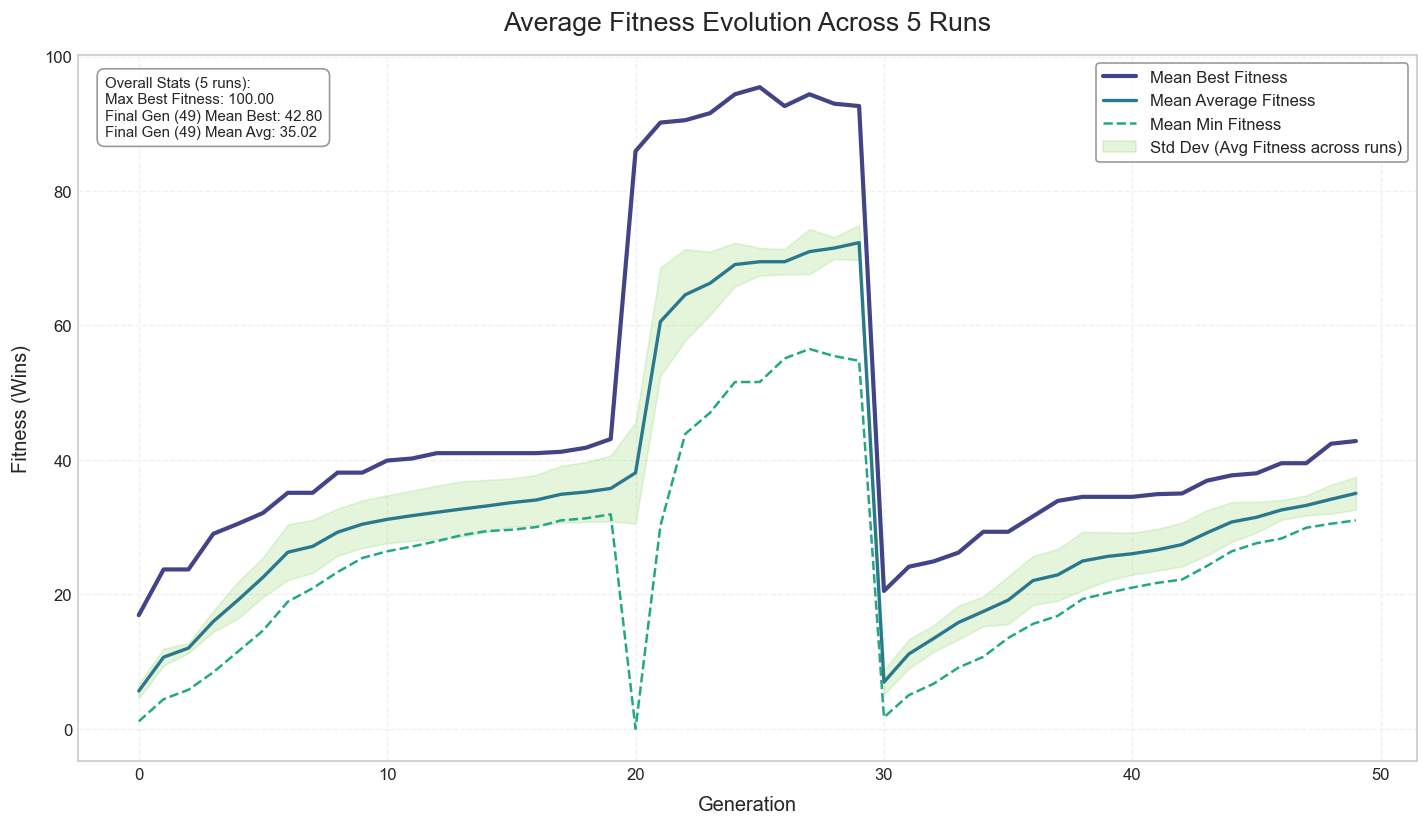
\includegraphics[width=1.0\textwidth]{img/424_fitness_evolution.png}
	\caption{Evolución del fitness sobre las generaciones para la combinación híbrida ganadora.}
	\label{fig:fitness_evolution_424}
\end{figure}

Este comportamiento también se refleja en los pesos de la población a lo largo de las generaciones, como se muestra en la figura \ref{fig:heat_avg_424}. En esta gráfica, en el eje x se muestran las mismas generaciones que en la figura anterior, mientras que en el eje y ahora se muestran los valores medios (a nivel de población) de los 20 pesos de cada bot. Como están normalizados, sus valores van desde 0, con un tono morado, hasta 1, con un tono amarillo. De nuevo, en las generaciones 20 y 30 se observa una especie de reseteo de la población, donde la mayoría de los individuos escogidos serían los hijos de la generación anterior y no sus padres, de ahí que los valores de los pesos parezcan cambiar de forma tan drástica.

Esta gráfica también se puede utilizar para identificar la forma en la que la población le da más o menos prioridad a cada uno de los pesos (tabla de significados en el capítulo \ref{chap:software_bot}). De hecho, fue una de las gráficas más importantes para determinar como se debía ajustar el uso y el cálculo de los pesos en el bot a lo largo del desarrollo de este proyecto. En cierto modo, está mostrando si a la población le ``gusta'' o no usar cada uno de ellos. Por ejemplo, el peso en el que más de acuerdo está la población de que debe ser muy bajo es el de \texttt{C\_TIER\_TAVERN}. Este peso es el que implementa una penalización por dejar cartas disponibles para su compra en la taberna. Cuanto mayor es la calidad de la carta, mayor es la penalización, la cual se va acumulando con cada carta. Tiene sentido que el valor de este peso sea muy bajo, ya que la suma de las penalizaciones de cada carta podría acabar siendo menor que el resto de pesos, desvirtualizando por completo la evaluación del fitness.

Otras valores interesantes pueden ser el de \texttt{POWER\_AMOUNT}, que simplemente le da un valor al cambio de poder entre cada acción. Es un peso extremadamente importante, puesto que el poder sobrante al terminar el turno se convierte en prestigio, la forma más usual de ganar una partida. Por último, destacar el incipiente uso de \texttt{T\_IMPRISONMENT} durante la etapa de coevolución. Parece que la población descubrió el uso de esta carta, pero acabó olvidándolo con el paso a la fase de modo fijo.

\begin{figure}[H]
	\centering
	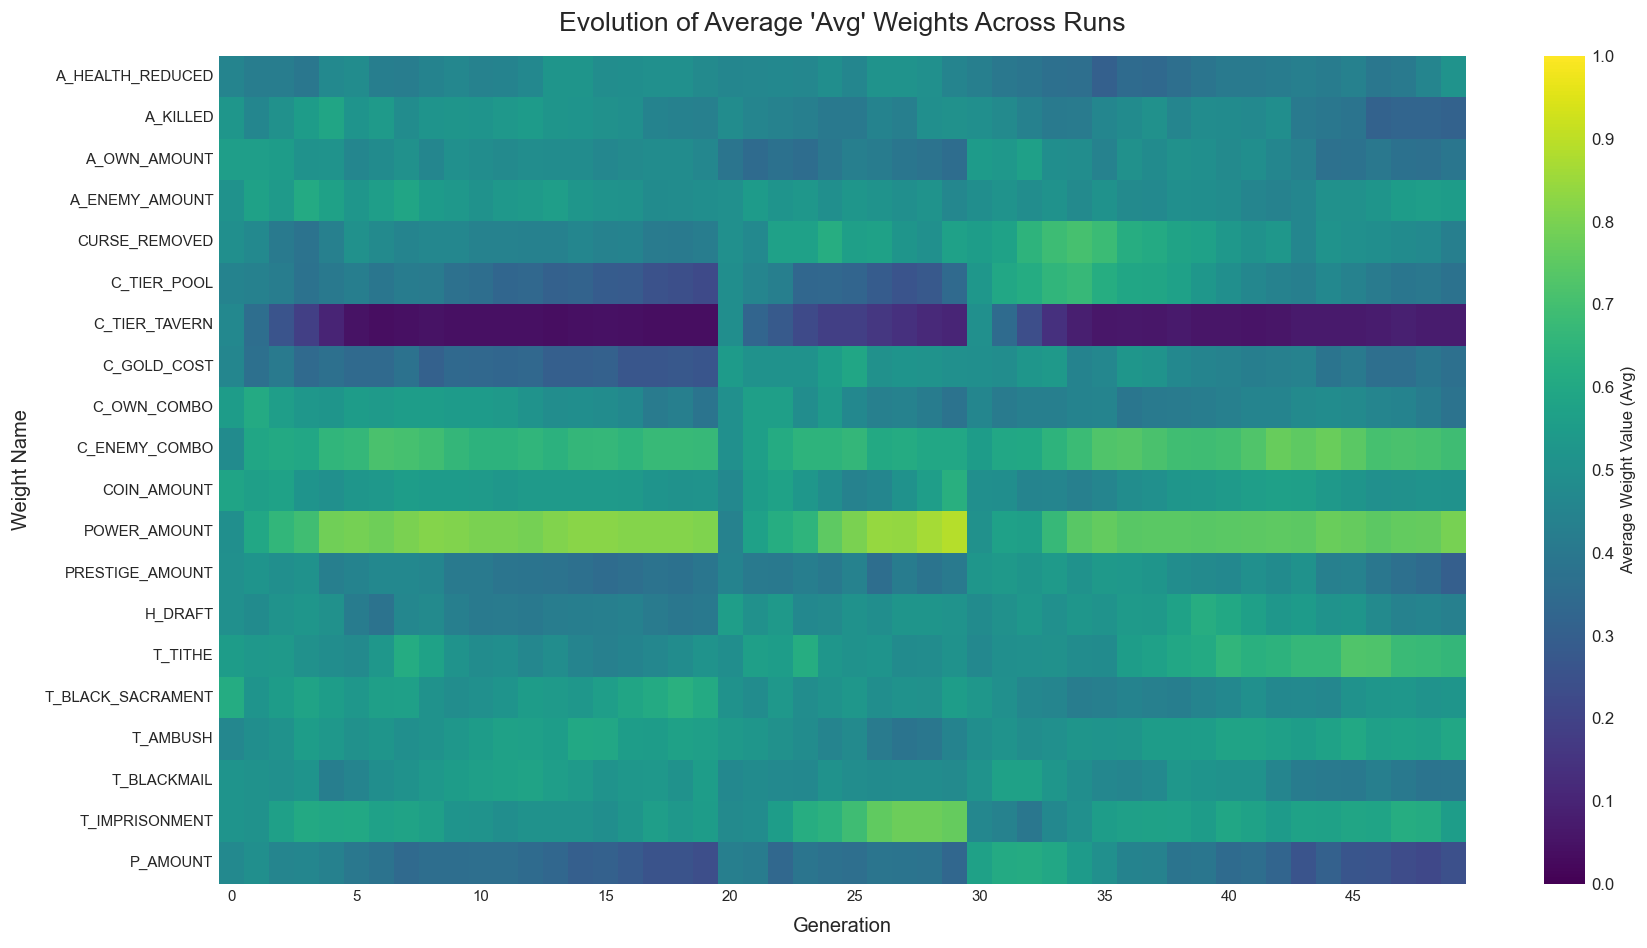
\includegraphics[width=1.0\textwidth]{img/424_heat_avg.png}
	\caption{Evolución de los pesos de la población a lo largo de las generaciones.}
	\label{fig:heat_avg_424}
\end{figure}

En definitiva, el análisis de las configuraciones híbridas revela que no existe una única fórmula para el éxito, pero sí una tendencia clara: las estrategias que logran un balance entre la explotación del conocimiento y la exploración de nuevas tácticas obtienen los mejores resultados. La configuración ganadora, H-3, sugiere que un enfoque que comienza y termina con una fase de entrenamiento guiado, intercalando una fase más corta de competición interna, resulta especialmente efectivo. Sin embargo, el buen rendimiento de la configuración H-5, dominada por la coevolución, demuestra que también es posible alcanzar un alto rendimiento partiendo de una exploración más abierta. Los resultados de los pesos, visibles en el mapa de calor, refuerzan esta idea, mostrando cómo la población aprende a priorizar ciertas heurísticas, como la importancia del poder o el descarte de cartas de bajo valor, adaptando su estrategia general en función de la naturaleza del desafío al que se enfrenta en cada fase del entrenamiento.

\section{Análisis de los modos de entrenamiento} \label{sec:analisis_modos_entrenamiento}

Tras la ejecución del conjunto experimental que compara los modos de entrenamiento y el salón de la fama (detallada en la Tabla \ref{tab:main_experiments}), se obtuvieron 6 campeones finales, uno por cada configuración evaluada. Para determinar de forma concluyente el rendimiento relativo de cada uno, se llevaron a cabo en este caso dos torneos finales, uno contra bots de referencia y otro entre sí mediante un emparejamiento estilo Round Robin. El primer torneo tuvo exactamente las mismas características que el realizado en la sección anterior, cada bot se enfrentó 5000 veces contra cada uno de los 4 bots de referencia, la mitad como jugador 1 y la otra como jugador 2. La Tabla \ref{tab:resultados_exp_modos} resume el rendimiento de cada campeón, ordenados de mayor a menor según su tasa de victorias global.

\begin{table}[H]
	\centering
	\caption{Rendimiento de los campeones de cada modo de entrenamiento contra oponentes fijos.}
	\label{tab:resultados_exp_modos}
    \small
	\begin{tabular}{@{}lccccccc@{}}
		\toprule
		\textbf{ID} & \textbf{Modo} & \textbf{Tasa Vic.} & \textbf{Tiempo} & \textbf{Patron} & \textbf{Agents} & \textbf{Prestige} & \textbf{Tree}   \\
		\midrule
		B-1         & Fijo F.       & \textbf{50.89\%}   & 2h 53m          & 68.6\%          & \textbf{76.8\%} & 34.1\%            & 24.1\%          \\
		B-5         & Híbrido       & 48.36\%            & 2h 39m          & \textbf{69.8\%} & 65.4\%          & 34.6\%            & 23.7\%          \\
		B-4         & Fijo          & 48.27\%            & \textbf{2h 27m} & 62.0\%          & 63.2\%          & 44.7\%            & 23.3\%          \\
		B-2         & Híbrido  F.   & 41.68\%            & 2h 48m          & 62.9\%          & 57.9\%          & 22.6\%            & 23.2\%          \\
		B-6         & Coevo.        & 35.01\%            & 2h 34m          & 44.0\%          & 21.1\%          & 50.1\%            & \textbf{24.8\%} \\
		B-3         & Coevo. F.     & 32.48\%            & 3h 11m          & 43.7\%          & 17.2\%          & \textbf{52.0\%}   & 17.0\%          \\
		\bottomrule
	\end{tabular}
\end{table}


El campeón del torneo contra los agentes de \textit{Scripts of Tribute} fue el B-1, que logró una tasa de victorias del 50.89\%. Este bot fue entrenado en modo fijo con el salón de la fama activado, lo que significa que los individuos de su población aspiraban constantemente a superar a los campeones de generaciones pasadas. Siguiéndole muy de cerca, los bots B-5 y B-4, que se entrenaron en modo híbrido y fijo respectivamente, lograron tasas de victorias del 48.36\% y 48.27\%. El B-5, es el ganador del torneo de configuraciones híbridas, lo que demuestra que este modo de entrenamiento es capaz de generar individuos competitivos incluso en un entorno con oponentes fijos. Por otro lado, el B-4, que se entrenó en modo fijo sin salón de la fama, demuestra que el modo fijo realmente es el más indicado para este tipo de torneo pues se basa en los mismos pasos que la población de este bot llevó a cabo durante su entrenamiento. Lo curioso es que parece que el salón de la fama en el modo híbrido no solo no aportó un beneficio, sino que incluso pudo haber perjudicado negativamente al rendimiento del bot, ya que el B-2, que también fue entrenado en modo híbrido pero con salón de la fama, obtuvo una tasa de victorias un 7.21\% inferior. Una posible explicación para este fenómeno es que el salón de la fama podría haber estado lleno de campeones que, si bien eran buenos en un segmento, no lo eran en el siguiente. Esto, en cierto modo, estaba confundiendo los valores la tasa de victoria final, asignándole un valor más alto a los individuos centrados en las tácticas válidas para el anterior segmento coevolutivo o fijo, pero no en el actual.

% Siguiente: hablar del tiempo de entrenamiento.

% --------------------

Para complementar la evaluación anterior, se realizó un segundo benchmark en formato de torneo coevolutivo. En esta fase, los 6 campeones se enfrentaron entre sí en una liguilla de todos contra todos, jugando 5,000 partidas en cada emparejamiento. Este tipo de validación es fundamental para medir la capacidad de un agente para adaptarse y superar a otros oponentes que también han evolucionado, en lugar de depender únicamente de explotar las debilidades de bots con estrategias fijas.

La Tabla \ref{tab:coevo_benchmark_resultados} presenta la matriz de resultados de este torneo, mostrando la tasa de victorias de cada campeón (en filas) contra cada oponente (en columnas). Adicionalmente, la Tabla \ref{tab:coevo_ranking_final} ofrece un resumen final, ordenando a los campeones según su rendimiento global en este entorno competitivo.

\begin{table}[H]
	\centering
	\caption{Matriz de resultados del torneo EvolutionaryBot vs EvolutionaryBot.}
	\label{tab:coevo_benchmark_resultados}
	\begin{tabular}{@{}lcccccc@{}}
		\toprule
		\textbf{vs}  & \textbf{B-1} & \textbf{B-2} & \textbf{B-3} & \textbf{B-4} & \textbf{B-5} & \textbf{B-6} \\
		\midrule
		\textbf{B-1} & ---          & 41.5\%       & 22.0\%       & 40.4\%       & 47.5\%       & 23.4\%       \\
		\textbf{B-2} & 58.5\%       & ---          & 3.4\%        & 44.6\%       & 51.3\%       & 4.3\%        \\
		\textbf{B-3} & 78.0\%       & 96.6\%       & ---          & 99.3\%       & 77.2\%       & 61.1\%       \\
		\textbf{B-4} & 59.6\%       & 55.4\%       & 0.7\%        & ---          & 50.8\%       & 3.4\%        \\
		\textbf{B-5} & 52.5\%       & 48.7\%       & 22.8\%       & 49.2\%       & ---          & 26.6\%       \\
		\textbf{B-6} & 76.6\%       & 95.7\%       & 38.9\%       & 96.6\%       & 73.4\%       & ---          \\
		\bottomrule
	\end{tabular}
\end{table}

\begin{table}[H]
	\centering
	\caption{Clasificación final del torneo EvolutionaryBot vs EvolutionaryBot.}
	\label{tab:coevo_ranking_final}
	\begin{tabular}{@{}lccc@{}}
		\toprule
		\textbf{ID} & \textbf{Modo} & \textbf{Tasa Vic.} & \textbf{Vic. Totales} \\
		\midrule
		B-3         & Coevo. F.     & 82.43\%            & (20607 / 25000)       \\
		B-6         & Coevo.        & 76.25\%            & (19063 / 25000)       \\
		B-5         & Híbrido       & 39.97\%            & (9992 / 25000)        \\
		B-1         & Fijo F.       & 34.95\%            & (8738 / 25000)        \\
		B-4         & Fijo          & 33.98\%            & (8494 / 25000)        \\
		B-2         & Híbrido F.    & 32.42\%            & (8106 / 25000)        \\
		\bottomrule
	\end{tabular}
\end{table}

\section{Análisis del salón de la fama} \label{sec:analisis_salon_fama}




% Decir que se han cumplido los dos objetivos faltantes:
% OG5: Evaluar cuantitativamente el rendimiento del agente entrenado mediante las diferentes estrategias, utilizando métricas relevantes.
% OG6: Analizar comparativamente la efectividad y eficiencia de las estrategias de optimización implementadas, discutiendo sus ventajas y desventajas en el contexto específico de ``Scripts of Tribute''.
% Decir que así concluye el cumplimiento de todos los objetivos específicos del proyecto.



